% \paragraph{Inference-Time Compute Techniques:} Inference-time compute involves using extra computational resources during inference time to improve the accuracy of language models.~\citep{snell2024scalingllmtesttimecompute,sumers2023cognitive,liu20251bllmsurpass405b,yang2025thinkingoptimalscalingtesttimecompute} For example, language models can produce intermediate outputs or reasoning steps before arriving at a final answer~\citep{wang2023selfconsistencyimproveschainthought,wei2023chainofthoughtpromptingelicitsreasoning}. Alternatively, compositional language model techniques compose multiple models at inference time to achieve better performance than a single model~\citep{li2024agentsneed,yin2024aggregationreasoninghierarchicalframework}.

% Producing intermediate outputs at inference time has been shown to significantly enhance smaller-scale models' performance~\citep{liu20251bllmsurpass405b}. However, existing research in compositional language models mostly focus on designing new methods using state-of-the-art LLMs~\citep{du2023improvingfactualityreasoninglanguage,khattab2023dspycompilingdeclarativelanguage,wu2023autogen}. However, whether smaller-scale models can benefit significantly from compositional methods remains an open question and is currently underexplored. Our work attempts to address this issue.

% \cw{TODO add a discussion based method definition}

% \paragraph{Compositional Language Models:} Compositional language models involve multiple language models working together to produce better results than a single model could achieve alone~\citep{jiang2023llmblenderensemblinglargelanguage,li2025rethinkingmixtureofagentsmixingdifferent,mitra2024distributedmixtureofagentsedgeinference}. By interacting and cooperating, these models combine their individual strengths through structured processes, including collaborative reasoning, critique, and verification, improving the quality of their final outputs~\citep{liang2024encouragingdivergentthinkinglarge,shinn2023reflexionlanguageagentsverbal,park2024ensemblinglargelanguagemodels,chen2025harnessingmultiplelargelanguage,khan2024debatingpersuasivellmsleads,gou2024criticlargelanguagemodels,mousavi2023ncriticsselfrefinementlargelanguage,gu2025surveyllmasajudge}. For example, LLM-Debate involves language models debating and critiquing each other to refine their final answers~\citep{du2023improvingfactualityreasoninglanguage}; Mixture-of-Agents synthesizes outputs from different models to produce comprehensive results~\citep{wang2024mixtureofagentsenhanceslargelanguage}; Multi-Agent Verification uses multiple models to independently evaluate candidate answers from different aspects and collectively select the best answer~\citep{lifshitz2025multiagentverificationscalingtesttime}. Figure~\ref{fig:comparison-methods} illustrates the workflow of these three methods. Despite the success of these methods, prior studies have primarily focused on composing frontier LLMs, while the composition of small-sized LLMs remains unexplored.

% Besides developing new frameworks, recent research has started optimizing existing compositional methods. Some studies focus on examining and optimizing model selection within these frameworks to improve their performance~\citep{li2025rethinkingmixtureofagentsmixingdifferent,chen2025optimizingmodelselectioncompound}. Other researchers try to enhance efficiency by improving the workflows or interaction designs of these methods. However, these efficiency improvements typically target specific methods rather than offering universally applicable solutions~\citep{li2024smoaimprovingmultiagentlarge,li2024improvingmultiagentdebatesparse,liu2024dynamicllmpoweredagentnetwork}.

\begin{figure}[t!]
    \centering
    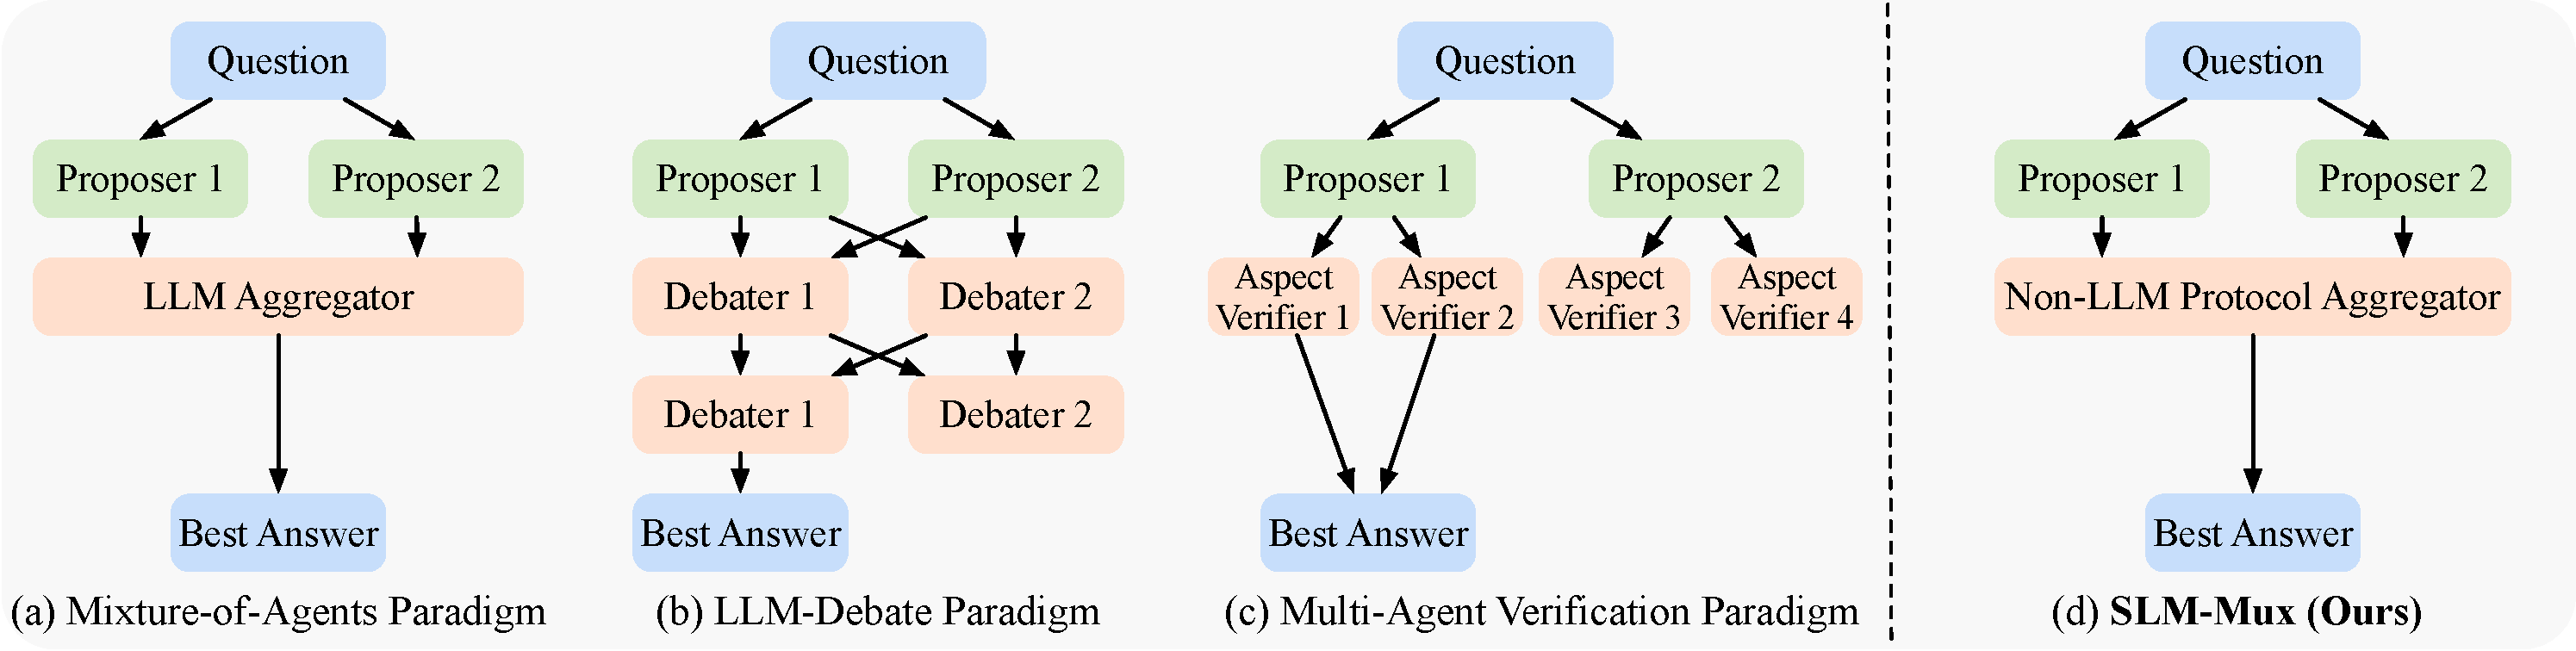
\includegraphics[width=\textwidth]{Figures/comparison_v3.pdf}
    \vspace{-10.5pt}
    \caption{\small \textbf{Comparing SLM-Mux (Ours) with Existing LLM Orchestration Methods.} (a) Mixture-of-Agents, (b) LLM-Debate, (c) Multi-Agent Verification, (d) SLM-Mux (Ours).}
    
    \label{fig:comparison-methods}
    % \vspace{-5pt}
\end{figure}

% \paragraph{Language Models Architectures Optimization}
% A growing body of work has explored engineering and orchestrating multiple LLMs into a single inference-time workflow. On the framework side, several systems allow users to design customized architectures~\citep{chen2023agentversefacilitatingmultiagentcollaboration,hong2024metagptmetaprogrammingmultiagent,shen2023hugginggptsolvingaitasks,li2023camelcommunicativeagentsmind}. For example, Autogen supports multi-agent conversation and tool integration~\citep{wu2023autogenenablingnextgenllm,schick2023toolformerlanguagemodelsteach}; and OpenAgents offers a deployable platform for data, web, and plugin-based agents~\citep{xie2023openagentsopenplatformlanguage}. 

% On the optimization side, prior work has focused on improving these compound LLM architectures, either by refining prompts or by searching for optimal workflows that guide LLMs to produce stronger outputs~\citep{khattab2023dspycompilingdeclarativelanguage,fernando2023promptbreederselfreferentialselfimprovementprompt,zhang2025aflowautomatingagenticworkflow,saadfalcon2025archonarchitecturesearchframework,opsahlong2024optimizinginstructionsdemonstrationsmultistage}. However, such approaches generally assume models with strong instruction-following abilities that are compatible with discussion-based frameworks. This assumption does not hold in our setting, which uses small-sized LLMs. Another line of work addresses model selection within compound LLM architectures~\citep{chen2025optimizingmodelselectioncompound,poon2025online}, but these approaches typically optimize only considering individual model accuracy without considering heterogeneity in model abilities. This limitation also makes them unsuitable for our setting.



% \paragraph{Test-time Scaling}
% Test-time scaling refers to methods that use extra computational resources during inference to boost model performance without retraining~\citep{snell2024scalingllmtesttimecompute,muennighoff2025s1simpletesttimescaling,zhang2025surveytesttimescalinglarge}. One line of work focuses on sampling multiple outputs from LLMs~\citep{chen2023universalselfconsistencylargelanguage,ichihara2025evaluationbestofnsamplingstrategies}. For example, self-consistency queries the model several times and uses the diversity of responses to estimate confidence, often improving accuracy~\citep{Trad_2025,thirukovalluru2024atomicselfconsistencybetterlong,chow2024inferenceawarefinetuningbestofnsampling}. However, most existing studies focus on a single model, whereas our work lies in the largely unexplored direction of combining the complementary strengths of multiple LLMs. 

% Another line of work encourages LLMs to spend more time reasoning before giving a final answer~\citep{wei2023chainofthoughtpromptingelicitsreasoning,yao2023treethoughtsdeliberateproblem,Besta_2024,dohan2022languagemodelcascades}. However, these approaches require further training of LLMs, which limits their flexibility across diverse use cases. In contrast, our method can directly utilize off-the-shelf models without additional training.

% However, test-time compute has limits. As the compute budget increases, performance eventually plateaus~\citep{dohan2022languagemodelcascades,chen2024llmcallsneedscaling}. The ceiling is determined by the capability of the underlying base model~\citep{chu2025ssrspeculativeparallelscaling,wu2025inferencescalinglawsempirical}. These limits motivate exploring more efficient and effective ways to compose multiple base LLMs at test time.

\paragraph{Discussion-based Orchestration Methods} We use discussion-based orchestration to refer to orchestration schemes where multiple LM instances exchange or evaluate natural-language messages—such as proposing answers, critiquing or debating, verifying from different aspects, and finally aggregating into one output. Representative approaches include Mixture-of-Agents~\citep{wang2024mixtureofagentsenhanceslargelanguage}, which uses a dedicated LLM to aggregate outputs from several models; LLM-Debate~\citep{du2023improvingfactualityreasoninglanguage}, where models critique and refine each other’s reasoning; and Multi-Agent Verification~\citep{lifshitz2025multiagentverificationscalingtesttime}, which assigns models to independently evaluate candidate solutions before selecting the final answer. These methods assume that participating models have sufficient reasoning ability to self-correct through interaction. Prior evaluations have been conducted on frontier LLMs, while their effectiveness for SLMs remains unstudied.

\looseness=-1
\paragraph{Optimization for Multi-LM Orchestration} Given these orchestration methods, some works study how to further improve their performance—e.g., how to select models to include, how to optimize prompts, or how to adapt the architecture for specific tasks~\citep{chen2023frugalgptuselargelanguage,ong2025routellmlearningroutellms,chen2024routerdcquerybasedrouterdual}. Prompt and workflow optimization methods~\citep{khattab2023dspycompilingdeclarativelanguage,opsahlong2024optimizinginstructionsdemonstrationsmultistage,saadfalcon2025archonarchitecturesearchframework, zhang2025aflowautomatingagenticworkflow} generally assume strong instruction-following ability, which makes them less effective for smaller models.

Another line of work is model selection for orchestration~\citep{chen2025optimizingmodelselectioncompound,poon2025online}. These methods often assume that models with higher standalone accuracy will yield stronger orchestrations. However, such strategies overlook conflicts among models: overconfident but incorrect predictions can dominate and suppress correct ones. Moreover, most selection criteria are not end-to-end—they evaluate models individually without directly assessing the performance of the orchestration itself. 

\paragraph{Test-time Scaling Strategies}
Test-time scaling refers to methods that improve performance by using additional computation during inference without retraining~\citep{snell2024scalingllmtesttimecompute,muennighoff2025s1simpletesttimescaling,zhang2025surveytesttimescalinglarge}. For a single model, a common approach is self-consistency~\citep{Trad_2025,thirukovalluru2024atomicselfconsistencybetterlong,chow2024inferenceawarefinetuningbestofnsampling}, where multiple samples are drawn and the majority answer is selected; accuracy typically improves as the number of samples increases. Extending this idea to multiple models, Agent Forest~\citep{li2024agentsneed} asks each model to produce one output and then applies majority voting over the pool of answers.